\documentclass{elegantbook}
\usepackage[square,numbers,sort&compress]{natbib}
\newcommand{\upcite}[1]{\textsuperscript{\textsuperscript{\cite{#1}}}}
\usepackage{multirow}
\usepackage{color}
\usepackage{tikz}
\usepackage{algorithm}
\usepackage{algorithmicx}
\usepackage{algpseudocode}
\usepackage{subfigure}
\renewcommand{\algorithmicrequire}{\textbf{Input: }}
\renewcommand{\algorithmicensure}{\textbf{Output: }}
\usetikzlibrary{shapes.geometric, arrows}
\tikzstyle{startstop} = [rectangle, rounded corners, minimum width = 2cm, minimum height=1cm,text centered, draw = black, fill = red!40]
\tikzstyle{acti} = [rectangle, trapezium left angle=70, trapezium right angle=110, minimum width=5cm, minimum height=0.5cm, text centered, draw=black, fill = blue!40]
\tikzstyle{pool} = [rectangle, trapezium left angle=70, trapezium right angle=110, minimum width=2cm, minimum height=0.5cm, text centered, draw=black, fill = purple!40]
\tikzstyle{process} = [rectangle, minimum width=3cm, minimum height=1cm, text centered, draw=black, fill = green!50]
\tikzstyle{conv} = [rectangle, minimum width=3cm, minimum height=1cm, text centered, draw=black, fill = magenta!50]
\tikzstyle{loss} = [rectangle, rounded corners, minimum width = 2cm, minimum height=1cm,text centered, draw = black, fill = yellow!40]
\tikzstyle{arrow} = [->,>=stealth]

% title info
\title{Deep Learning}
\subtitle{Variational Auto-Encoders}
% bio info
\author{Yantian Luo}
\institute{Electronic Engineering}
\version{2018310742}
\date{\today}
\logo{logo.png}
\cover{cover.jpg}

\begin{document}

\maketitle
\tableofcontents
\mainmatter
\hypersetup{pageanchor=true}
% add preface chapter here if needed
\chapter{Introduction}
In this homework, we need to use Zhusuan to implement Variational Auto-Encoders. Let $x$ denote the observable data and $z$ denote the corresponding latent variable that can describe the data. The generative process of the Variational Auto-Encoders (VAEs) with Gaussian prior of $z$ and Bernoulli likelihood of $x$ is defined as follows:
\begin{equation}
\begin{aligned} z & \sim \mathcal{N}(\mathbf{0}, \mathbf{I}) \\ \mu_{x} &=f(z) \\ x & \sim \mathcal{B}\left(\mu_{x}\right) \end{aligned}
\end{equation}
where $\mathcal{N} (0, I)$ is the standard Gaussian distribution, $f$ is parameterized by a deep neural network and $\mathcal{B}(\mu_x )$ is the multivariate Bernoulli distribution. As in our case where $x$ is multi-dimensional, each dimension of $x$ is sampled independently given the corresponding dimension of $\mu_x$ following one-dimensional Bernoulli distribution.

Also we can define the generative process of the Variational Auto-Encoders (VAEs) with Gaussian prior of $z$ and Gaussian likelihood of $x$ as follows:
\begin{equation}
\begin{aligned} z & \sim \mathcal{N}(\mathbf{0}, \mathbf{I}) \\ \mu_{x} &=f_{\mu}(z) \\ \sigma_{x} &=f_{\sigma}(z) \\ x & \sim \mathcal{N}\left(\mu_{x}, \sigma_{x}\right) \end{aligned}
\end{equation}

Then to infer the latent variable $z$ given observable $x$, VAEs build a recognition model as follows:
\begin{equation}
\begin{aligned} \mu_{z} &=g_{\mu}(x) \\ \sigma_{z} &=g_{\sigma}(x) \\ z & \sim \mathcal{N}\left(\mu_{z}, \sigma_{z}\right) \end{aligned}
\end{equation}
where $g_\mu$ and $g_\sigma$ are parameterized as deepneural networks, which can share most of the parameters.

To jointly learn the parameters in all networks, VAEs defines a variational lower-bound of the marginal data
likelihood for per data, i.e. $p(x)$ and sums over them.

\chapter{VAE-Base Results}
In this chapter, we implement the code ``vae\_base.py'' and add code to randomly sample 100 latent variables $z$ from Gaussian prior and plot their corresponding images. We training for 10 epochs and draw the corresponding images as shown in Figure \ref{res2}. We can find that the generating images is similar with the true images. And we also draw the corresponding images for some epochs as shown in \ref{res1}, from the training process images, we can find that the images is getting clearer and more and more similar with true images.
\begin{figure}[!h]
	\centering
	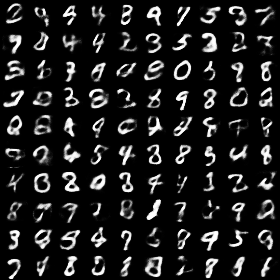
\includegraphics[width=0.8\linewidth]{../results/vae_epoch_10.png}
	\caption{\label{res2}The corresponding images after training}
\end{figure}
\begin{figure}[!h]
	\centering
	\subfigure[epoch=1]{ 
		\label{fig:subfig:a} %% label for first subfigure 
		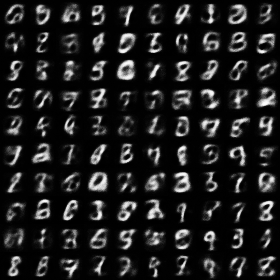
\includegraphics[width=0.4\linewidth]{../results/vae_epoch_1.png}} 
	\hspace{0.1in}
	\subfigure[epoch=3]{ 
		\label{fig:subfig:b} %% label for first subfigure 
		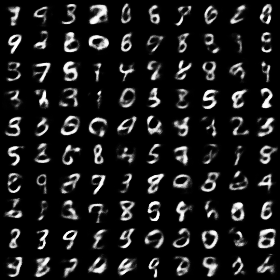
\includegraphics[width=0.4\linewidth]{../results/vae_epoch_3.png}} 
	\hspace{0.1in}
	\subfigure[epoch=5]{ 
		\label{fig:subfig:c} %% label for first subfigure 
		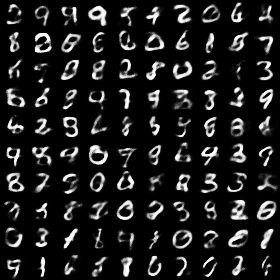
\includegraphics[width=0.4\linewidth]{../results/vae_epoch_5.png}} 
	\hspace{0.1in}
	\subfigure[epoch=7]{ 
		\label{fig:subfig:d} %% label for first subfigure 
		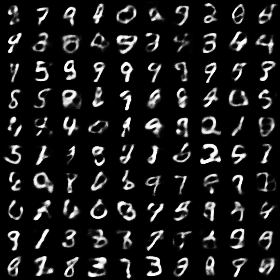
\includegraphics[width=0.4\linewidth]{../results/vae_epoch_7.png}} 
	\hspace{0.1in}
	\subfigure[epoch=8]{ 
		\label{fig:subfig:e} %% label for first subfigure 
		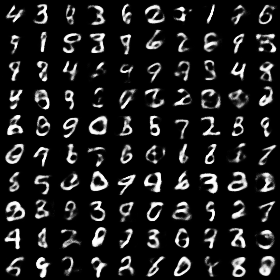
\includegraphics[width=0.4\linewidth]{../results/vae_epoch_8.png}} 
	\hspace{0.1in}
	\subfigure[epoch=9]{ 
		\label{fig:subfig:f} %% label for first subfigure 
		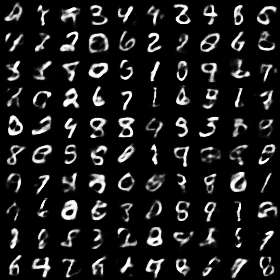
\includegraphics[width=0.4\linewidth]{../results/vae_epoch_9.png}} 
	\caption{\label{res1}The corresponding images for some epochs}
\end{figure}

\chapter{VAE-Gaussian Results}
\section{The Providing Codes}
In this section, we implement the code ``vae\_gaussian.py'' and add code to randomly sample 100 latent variables $z$ from Gaussian prior and plot their corresponding images. We training for 10 epochs and draw the corresponding images as shown in Figure \ref{res3}. We can find that the generating images much worse than Bernoulli likelihood case. The results may be that Bernoulli likelihood will bring some prior information to $x$ but Gaussian doesn't. And we also draw the corresponding images for some epochs as shown in \ref{res4}, from the training process images, we can find that the images is getting clearer but also not similar with true images in 10 epochs.
\begin{figure}[!h]
	\centering
	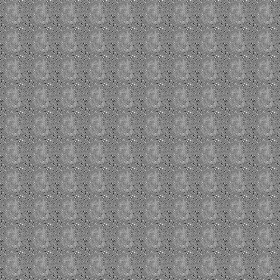
\includegraphics[width=0.8\linewidth]{../results/vae_gaussian_epoch_10.png}
	\caption{\label{res3}The corresponding images after training}
\end{figure}
\begin{figure}[!h]
	\centering
	\subfigure[epoch=1]{ 
		\label{fig:subfig:2a} %% label for first subfigure 
		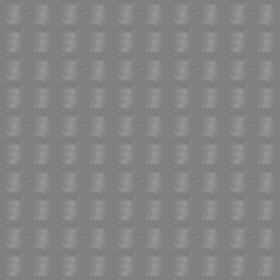
\includegraphics[width=0.4\linewidth]{../results/vae_gaussian_epoch_1.png}} 
	\hspace{0.1in}
	\subfigure[epoch=3]{ 
		\label{fig:subfig:2b} %% label for first subfigure 
		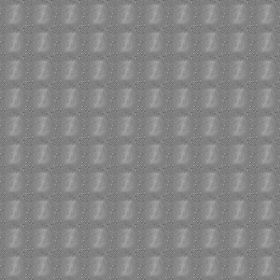
\includegraphics[width=0.4\linewidth]{../results/vae_gaussian_epoch_3.png}} 
	\hspace{0.1in}
	\subfigure[epoch=5]{ 
		\label{fig:subfig:2c} %% label for first subfigure 
		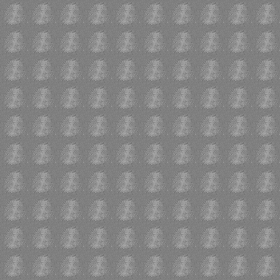
\includegraphics[width=0.4\linewidth]{../results/vae_gaussian_epoch_5.png}} 
	\hspace{0.1in}
	\subfigure[epoch=7]{ 
		\label{fig:subfig:2d} %% label for first subfigure 
		
\includegraphics[width=0.4\linewidth]{../results/vae_gaussian_epoch_7.png}} 
	\hspace{0.1in}
	\subfigure[epoch=8]{ 
		\label{fig:subfig:2e} %% label for first subfigure 
		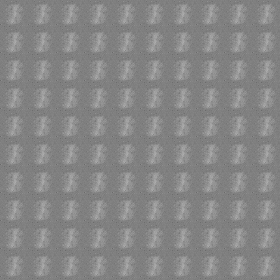
\includegraphics[width=0.4\linewidth]{../results/vae_gaussian_epoch_8.png}} 
	\hspace{0.1in}
	\subfigure[epoch=9]{ 
		\label{fig:subfig:2f} %% label for first subfigure 
		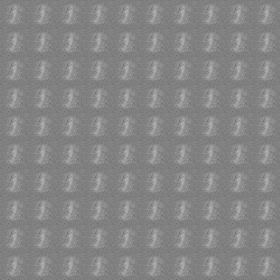
\includegraphics[width=0.4\linewidth]{../results/vae_gaussian_epoch_9.png}} 
	\caption{\label{res4}The corresponding images for some epochs}
\end{figure}
\section{Another implement}
According the results in the last section, we can find that the results is not very good. But I don't know whether the code is right. Therefore, in this section, we use codes in ``vae.py'' which is similar with the tutorial codes provided by zhusuan to implement. We training for 10 epochs and draw the corresponding images as shown in Figure \ref{res5}. We can find that in this implement, the results is better than the providing codes but also is worse than Bernoulli likelihood case. And we also draw the corresponding images for some epochs as shown in \ref{res4}, from the training process images, we can find that the images is getting clearer in 10 epochs.

\begin{figure}[!h]
	\centering
	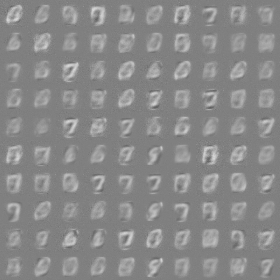
\includegraphics[width=0.8\linewidth]{../results/vae3_gaussian_epoch_10.png}
	\caption{\label{res5}The corresponding images after training}
\end{figure}
\begin{figure}[!h]
	\centering
	\subfigure[epoch=1]{ 
		\label{fig:subfig:3a} %% label for first subfigure 
		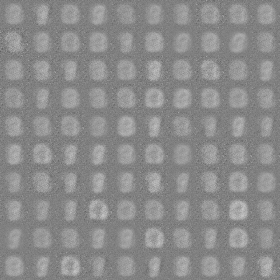
\includegraphics[width=0.4\linewidth]{../results/vae3_gaussian_epoch_1.png}} 
	\hspace{0.1in}
	\subfigure[epoch=3]{ 
		\label{fig:subfig:3b} %% label for first subfigure 
		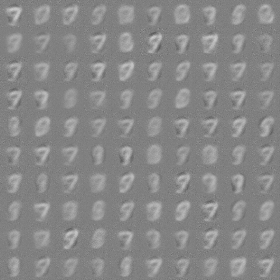
\includegraphics[width=0.4\linewidth]{../results/vae3_gaussian_epoch_3.png}} 
	\hspace{0.1in}
	\subfigure[epoch=5]{ 
		\label{fig:subfig:3c} %% label for first subfigure 
		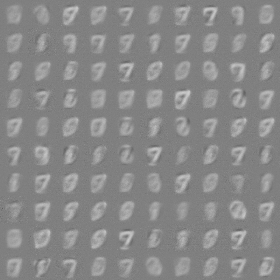
\includegraphics[width=0.4\linewidth]{../results/vae3_gaussian_epoch_5.png}} 
	\hspace{0.1in}
	\subfigure[epoch=7]{ 
		\label{fig:subfig:3d} %% label for first subfigure 
		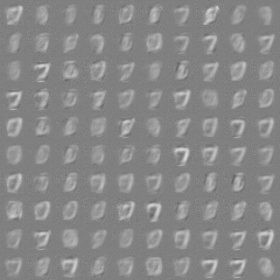
\includegraphics[width=0.4\linewidth]{../results/vae3_gaussian_epoch_7.png}} 
	\hspace{0.1in}
	\subfigure[epoch=8]{ 
		\label{fig:subfig:3e} %% label for first subfigure 
		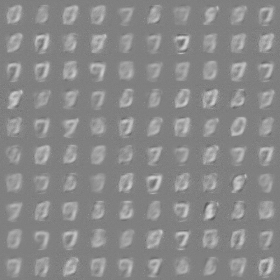
\includegraphics[width=0.4\linewidth]{../results/vae3_gaussian_epoch_8.png}} 
	\hspace{0.1in}
	\subfigure[epoch=9]{ 
		\label{fig:subfig:3f} %% label for first subfigure 
		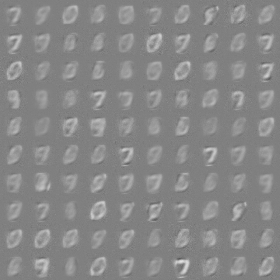
\includegraphics[width=0.4\linewidth]{../results/vae3_gaussian_epoch_9.png}} 
	\caption{\label{res6}The corresponding images for some epochs}
\end{figure}
\end{document}